
\chapter{Introduction}

Scientists, engineers, and researchers use wireless sensor networks (WSN) for a wide array of applications. Many of these applications rely on knowledge of the precise position of each node. While some may only require relative coordinates within the network, most biological, geophysical, and other scientific applications require coordinates on a global coordinate system. Perhaps the obvious solution is for each node in the network to be equipped with GPS or other location positioning services.  However, constraints on cost, power consumption, as well as visibility of satellites dictate the need for an alternative solution.  

Many protocols have been proposed\cite{APS,MDS-MAP,CCA-MAP07} to calculate relative positions amongst the nodes of a network.  They vary in the required network functionality in terms of radio ranging or range-free.  Radio ranging involves specialized hardware to measure the distance between nodes based on physical data like signal strength or transmission delays.  In order to convert from relative to global coordinates, some of the nodes require a local source of global coordinates.  This can be achieved by operators recording the global coordinates during network deployment, by embedding a GPS receiver in a subset of the nodes, or some other source.  We call these enhanced nodes anchors.  Here, we explore the effect of anchor node placement within the network on the overall localization errors, on a network-wide basis. This provides network planners with a set of general rules to minimize the number of anchor nodes required while avoiding poor node localization, allowing scientists to assume a maximum position error during their own research.  Further, based on application requirements of location accuracy, planners can minimize the cost of the network associated with anchor nodes by using the minimum number and best position.

\section{Motivation} 
\begin{figure}
  \centering
    \subfloat[Anchor Set 1]{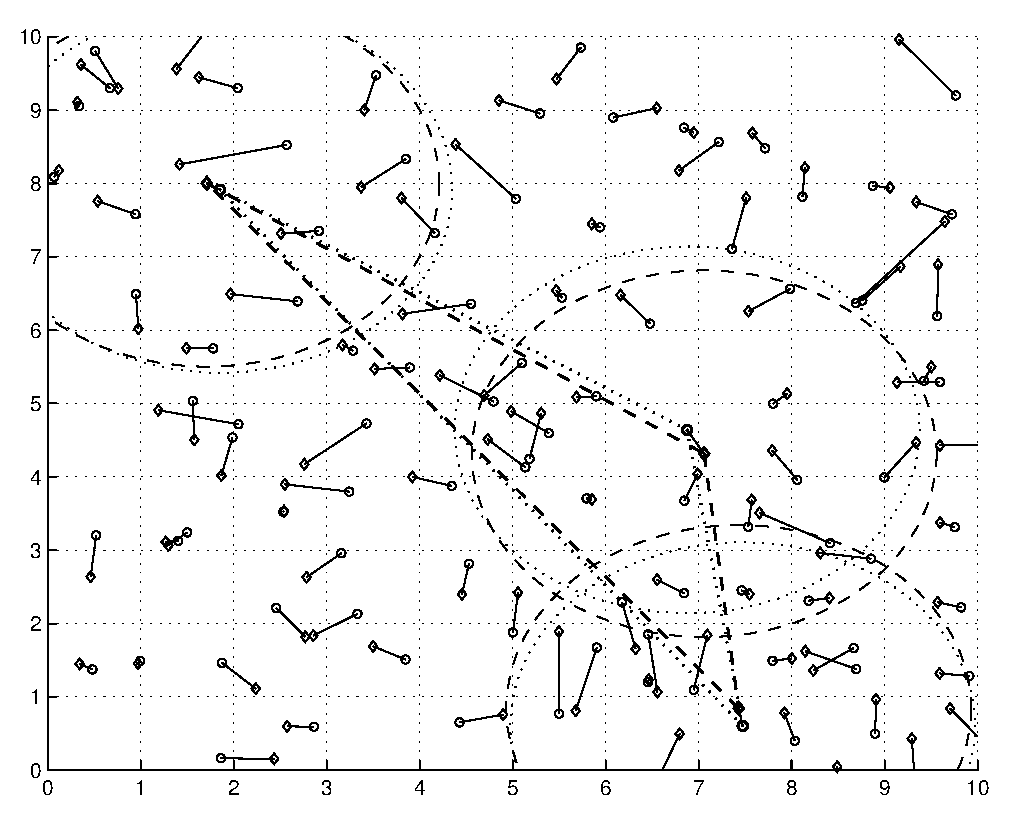
\includegraphics[width=\figurewidth\textwidth]{motivation/plot1}}\\
    \subfloat[Anchor Set 2]{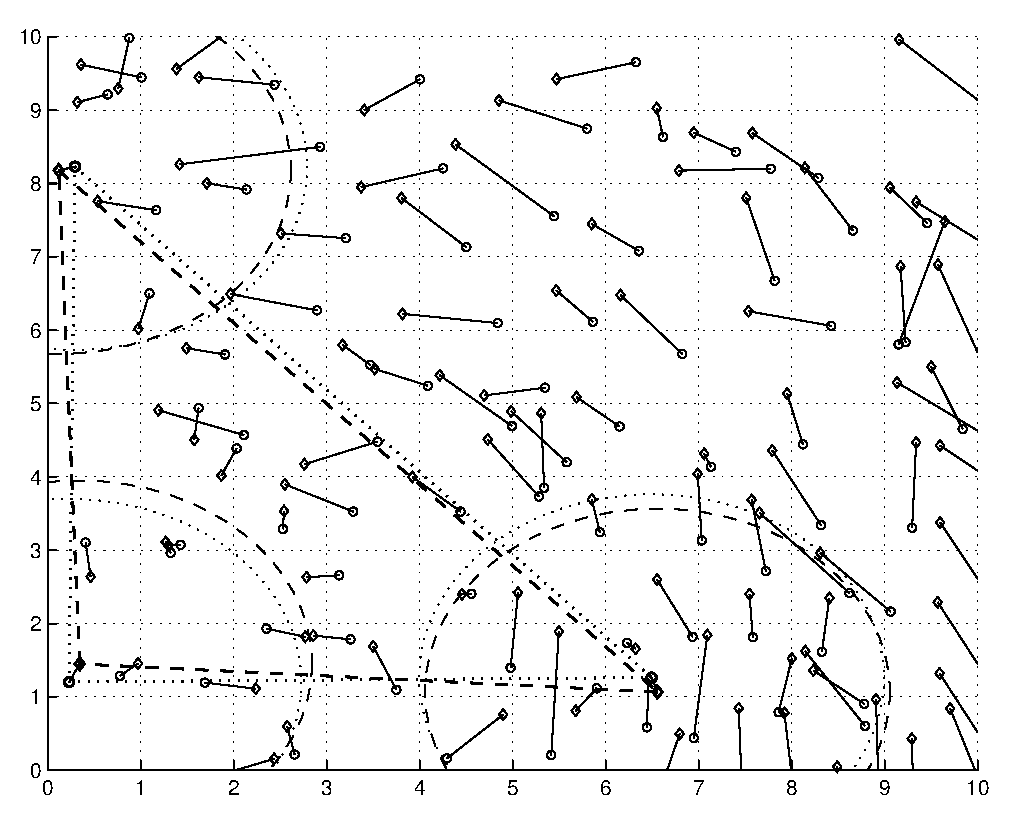
\includegraphics[width=\figurewidth\textwidth]{motivation/plot2}}
	\caption{Reasonable localization results}
    \label{fig:Motivation1}    
\end{figure}
\begin{figure}
  \centering
    \subfloat[Anchor Set 3]{\label{fig:Motivation2a}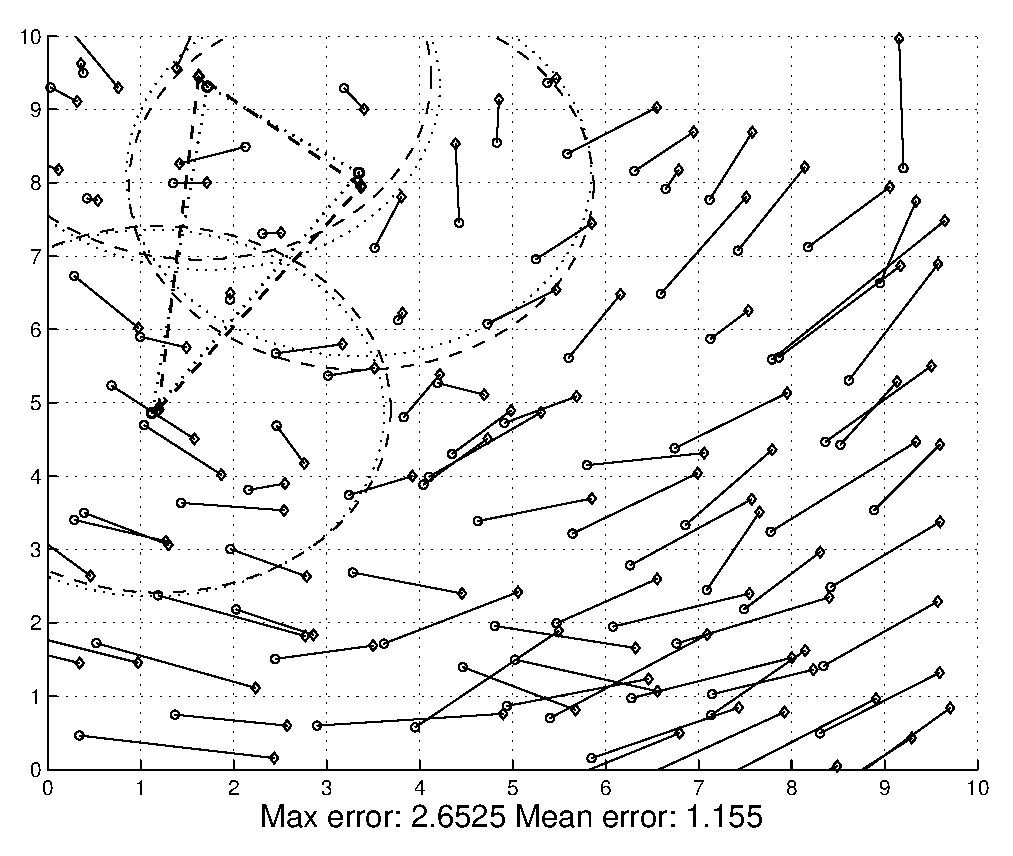
\includegraphics[width=\figurewidth\textwidth]{motivation/plot3}}
	\\
    \subfloat[Anchor Set 4]{\label{fig:Motivation2b}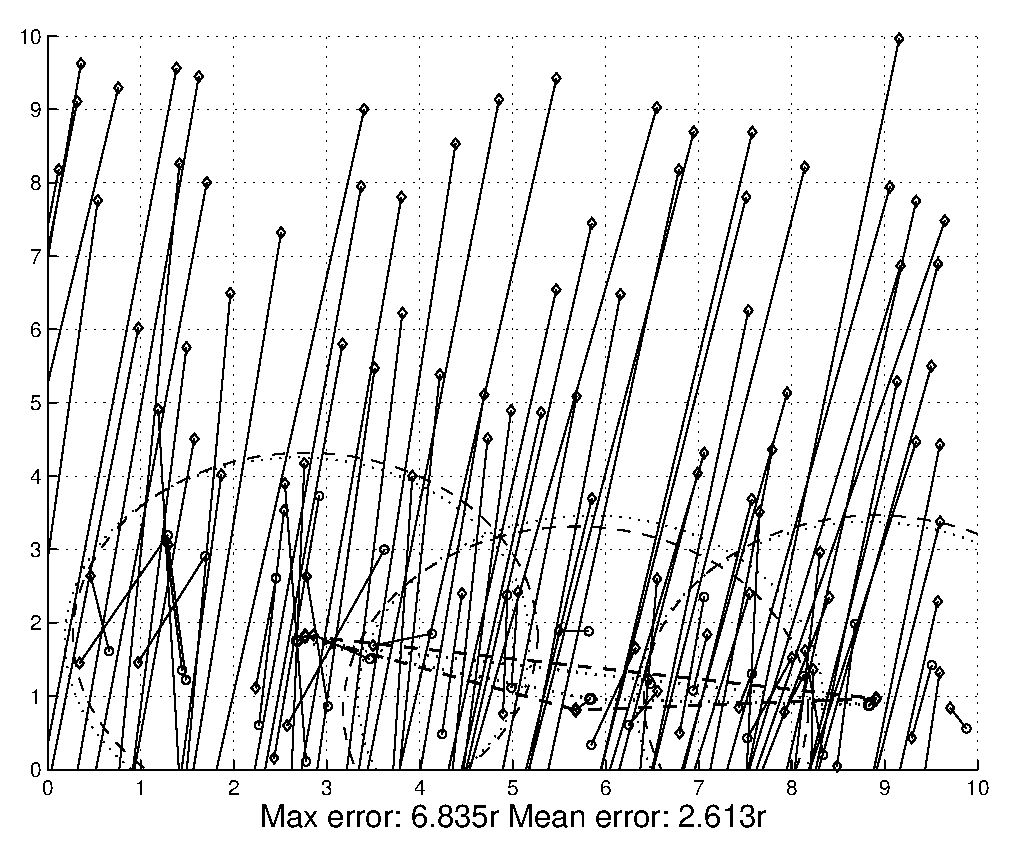
\includegraphics[width=\figurewidth\textwidth]{motivation/plot4}}
    \caption{Poor localization results}
    \label{fig:Motivation2}
\end{figure}

During previous work designing localization protocols\cite[p. 11]{CCA-MAP09}\cite[p.2 ]{MDS-MAP}, researchers often choose anchors at random within the network.  Frequently, they simulate the network multiple times with different anchors in order to statistically exclude anchor node placement from their results. 

Our initial investigations and simulations demonstrate that indeed the placement of anchor nodes in the network does have an often dramatic effect on the location error.  The four plots shown in Figures~\ref{fig:Motivation1} and \ref{fig:Motivation2} graphically establish that anchor node position does make a difference.  Each plot shows the same network with a different choice of three anchors.  A line is drawn between the actual and calculated position of each node to visualize the localization error.  The circles show the radio range of each anchor, and a triangle is drawn between the three anchors for clarity.  

The four plots shown are taken from a set of 100 randomly chosen anchor sets.  While the first two choices, shown in Figure~\ref{fig:Motivation1}, have reasonable errors, the third choice, in Figure~\ref{fig:Motivation2a}, has an error more than twice the mean error of the first.  Further, the fourth choice, in Figure~\ref{fig:Motivation2b}, has an extremely poor performance, more than ten times that of the first choice.  The four anchor set triangles shown do not immediately show an obvious progression that could explain this dramatic change in error. We find it interesting that there is an incremental increase in error between these four anchor sets resulting in a full order of magnitude difference between good and bad cases, and thus requires the further investigation presented in this thesis.

In practical applications, scientists and engineers need to know what degree of accuracy the localization algorithm provides. This study, therefore, diagnoses the impact of anchor node placement on these errors and, while providing guidelines for anchor node placement, establishes some bounds for the resulting error. 

\section{Thesis Contribution}
We establish that by avoiding certain poor anchor node placements, extremely poor location errors can be avoided.  Further, we demonstrate that other than these edge cases, the location error falls within a statistically insignificant range, where the range is a function of network connectivity and topology.  Specifically, we show that the probability of extremely high location error results from anchor nodes being roughly in a geographically straight line.  As the anchor nodes are spread out from a straight line, the probability of high errors decreases, leaving network designers a relatively simple chore when choosing anchor nodes locations.

While some papers have touched upon anchor node placement, we have yet to come across a comprehensive study of the optimal anchor node placement.  This paper provides a comprehensive study of possible anchor node placements and their effects on overall network localization accuracy.

While this paper is a comprehensive study of anchor node placements, we focus on a specific set of network design assumptions.  First, we assume the network planners want to minimize the number of anchors since they consume more power and cost more.  Therefore, we assume the minimum number of anchors of three to provide two-dimensional coordinates. Further, we assume that range-free algorithms are preferred to avoid dealing with multi-path and other radio effects as well as to limit the required hardware and power requirements on each node in the network.  

\section{Methodology}
Many localization protocols and algorithms provide a set of relative coordinates that are then transformed into global coordinates.  For the purpose of this research, we chose CCA-MAP\cite{CCA-MAP07,CCA-MAP09} as the algorithm to provide simulation results.  A Matlab\copyright~  simulation of this algorithm already existed\cite{CCA-MAP07}, and was modified to provide the necessary output statistics presented here.  CCA-MAP is described in more detail in Section~\ref{sec:CCA-MAP}.

\section{Thesis Organization}
A brief background of Wireless Sensor Networks and localization protocols in general are presented in Chapter 2.  Chapter 3 presents the limited related work on anchor node placement.  Chapter 4 contains various proposed anchor node placement methods and summaries of how they perform.  The cause of the extreme edge cases comes to light in Chapter 5.  Chapter 6 discusses various other factors. Chapter 7 gives some ideas for future work, including other factors that effect localization error and Chapter 8 summarizes the results of this study.

%\begin{equation}\label{eqn:newton_law} %    F = Ma %\end{equation}
%Paragraph referencing an equation \ref{eqn:newton_law}.
